\section{Software Controlador}

\subsection{Visão Geral}
\par O software de controle será capaz de mostrar o consumo energético, assim como realizar as operações desejadas pelo usuário.

\subsection{Requisitos do Software}

\subsubsection{Problema a Ser Resolvido}
\par O problema a ser solucionado pelo software está representado na seguinte tabela:

\begin{table}[h]
\captionof{table}{Descrição do Problema}
\centering
\begin{tabular}{|l|l|}
\hline
\multirow{\textbf{O problema seria}}        & a dificuldade de interação entre o usuário e o sistema \\
                                            & de automação \\ \hline
\multirow{\textbf{que afeta}}               & a usabilidade e acesso às informações por parte do \\
                                            & usuário \\ \hline
\multirow{\textbf{cujo impacto é}}          & impedir o usuário de usufruir de todas as funcionalidades \\
                                            & disponibilizadas pelo sistema \\ \hline
\multirow{\textbf{uma boa solução seria}}   & o desenvolvimento de um software que seja a interface \\
                                            & entre o usuário e o sistema, a fim de amenizar ao máximo \\
                                            & sua dificuldade de interagir com o sistema de automação. \\ \hline
\end{tabular}
\end{table}

\subsubsection{Requisitos Funcionais}
\par Foram levantados os seguintes requisitos funcionais relacionados ao funcionamento do software:

\begin{table}[h]
\captionof{table}{Descrição dos Requisitos Funcionais}
\centering
\begin{tabular}{|l|l|l|}
\hline
\textbf{ID}                 & \textbf{Descrição}                                & \textbf{Dependências} \\ \hline
\multirow{\textbf{RF01}}    & O sistema deve manter os registros de consumo     & N/A \\
                            & de recursos da residência.                        & \\ \hline
\multirow{\textbf{RF02}}    & O sistema deve apresentar relatórios sobre os     & RF01 \\
                            & registros de consumo de recursos da residência.   & \\ \hline
\multirow{\textbf{RF03}}    & O sistema deve receber e armazenar os dados dos   & RNF01 \\
                            & sensores presentes na residência.                 & \\ \hline
\multirow{\textbf{RF04}}    & O sistema deve permitir que o usuário mantenha    & RF01 \\
                            & metas de consumos de recursos da residência.      & \\ \hline
\multirow{\textbf{RF05}}    & O sistema deve exibir o feed de gravação das      & RNF01 \\
                            & câmeras de segurança interna à residência.        & \\ \hline
\multirow{\textbf{RF06}}    & O sistema deve manter as gravações das câmeras de & RF05 \\
                            & segurança interna pelo período de um mês após a   & \\
                            & gravação.                                         & \\ \hline
\end{tabular}
\end{table}

\begin{table}[h]
\centering
\begin{tabular}{|l|l|l|}
\hline
\textbf{ID}                 & \textbf{Descrição}                                & \textbf{Dependências} \\ \hline
\multirow{\textbf{RF07}}    & O sistema deve permitir que o usuário configure   & N/A \\
                            & backups automáticos.                              & \\ \hline
\multirow{\textbf{RF08}}    & O sistema deve notificar o usuário em caso de     & RNF01 \\
                            & princípio de incêndio.                            & \\ \hline
\multirow{\textbf{RF09}}    & O sistema deve permitir o usuário a criar modos   & N/A \\
                            & de vigilância de áreas da casa.                   & \\ \hline
\multirow{\textbf{RF10}}    & O sistema deve notificar o usuário caso o sensor  & RNF01 \\
                            & de presença seja acionado, de acordo com o modo   & RF09 \\
                            & de segurança atual.                               & \\ \hline
\multirow{\textbf{RF11}}    & O sistema deve notificar o usuário caso o sensor  & N/A \\
                            & de gás detecte a presença de gases prejudiciais.  & \\ \hline
\multirow{\textbf{RF12}}    & O sistema deve permitir que o usuário controle a  & N/A \\
                            & iluminação dos cômodos da residência pela         & \\
                            & interface.                                        & \\ \hline
\multirow{\textbf{RF13}}    & O sistema deve permitir que o usuário controle a  & N/A \\
                            & ativação/desativação dos aparelhos eletrônicos    & \\
                            & cadastrados pela interface.                       & \\ \hline
\end{tabular}
\end{table}

\subsubsection{Requisitos Não Funcionais}
\par Foram levantados os seguintes requisitos não funcionais relacionados ao funcionamento do software:

\begin{table}[h]
\captionof{table}{Descrição dos Requisitos Não Funcionais}
\centering
\begin{tabular}{|l|l|}
\hline
\textbf{ID}                 & \textbf{Descrição} \\ \hline
\multirow{\textbf{RNF01}}   & O sistema deve possuir conexão com os sensores de diversos tipos e    \\
                            & câmeras de vigilância presentes na residência durante todo o período  \\
                            & de funcionamento.                                                     \\ \hline
\multirow{\textbf{RNF02}}   & O sistema deve estar conectado à um servidor local à residência.      \\ \hline
\multirow{\textbf{RNF03}}   & O sistema de bancos de dados deve salvar as informações do sistema em \\
                            & uma base de dados criptografada com senha.                            \\ \hline
\end{tabular}
\end{table}

\subsection{Casos de Uso}

\subsubsection{Sobre os Casos de Uso}
\par Visando uma maior objetividade deste documento, o detalhamento dos casos de uso aqui apresentados encontra-se em anexo no documento de Especificações de Casos de Uso.

\subsubsection{Diagrama de Casos de Uso}

\begin{figure}[!ht]
\caption{Diagrama de Casos de Uso}
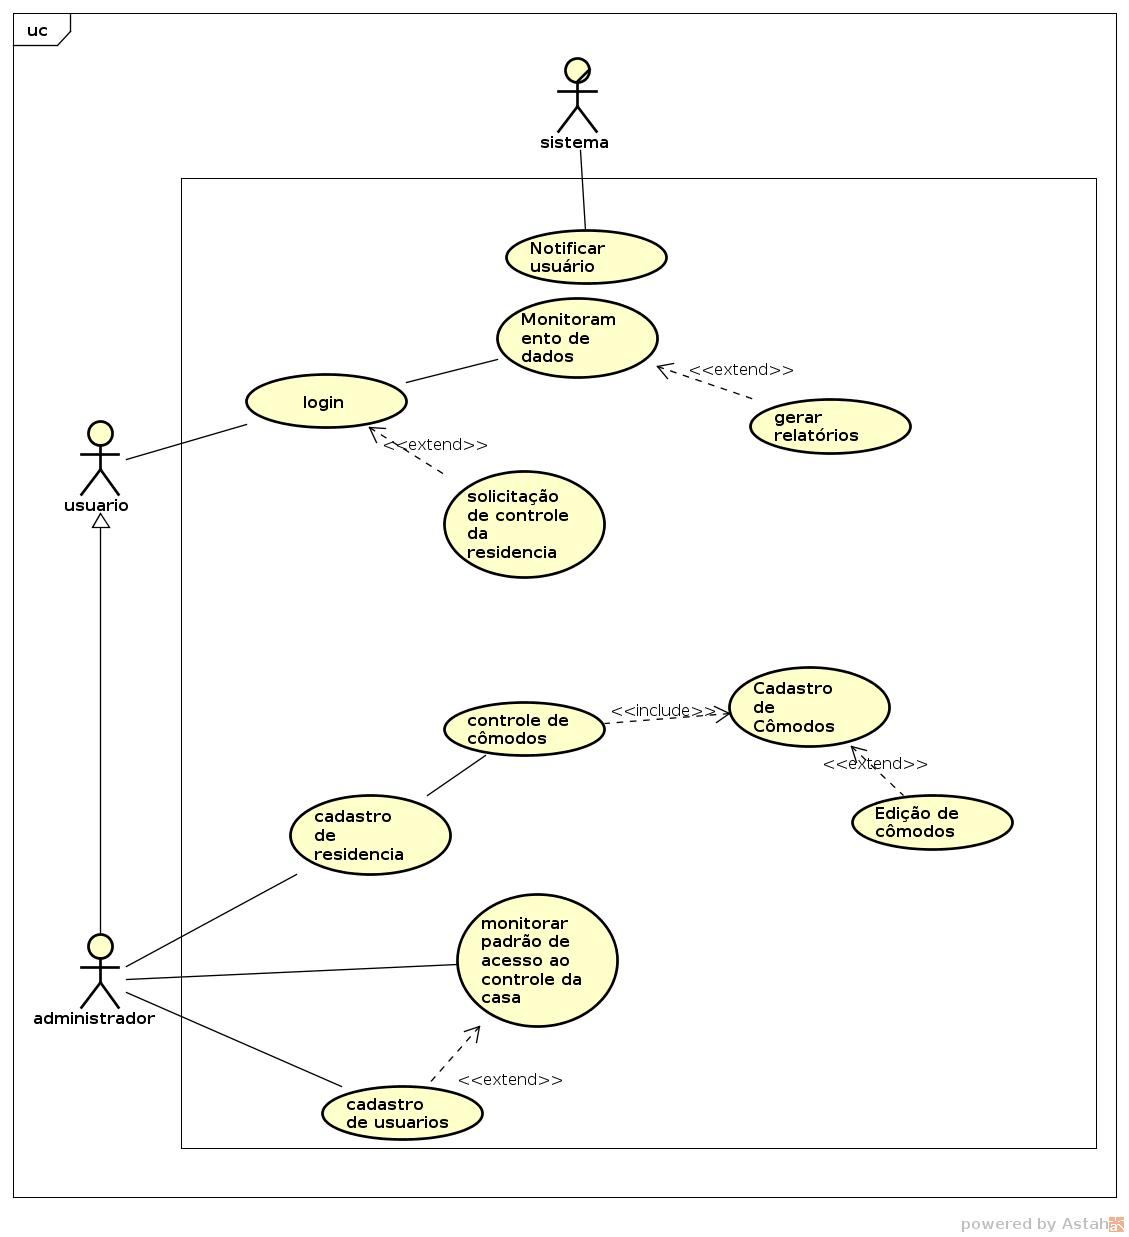
\includegraphics[width=\textwidth]{figuras/usecases}
\end{figure}

\newpage

\subsubsection{Descrição dos Casos de Uso}

\begin{table}[h]
\captionof{table}{Descrição dos Casos de Uso}
\centering
\begin{tabular}{|l|l|l|l|}
\hline
\textbf{ID}                 & \textbf{Nome}         & \textbf{Descrição}                & \textbf{Ator(es)} \\ \hline
\multirow{\textbf{UC01}}    & Login de Usuário      & Permite que um usuário cadastrado & Usuário           \\
                            &                       & efetue login no sistema.          &                   \\ \hline
\end{tabular}
\end{table}

\begin{table}[h]
\centering
\begin{tabular}{|l|l|l|l|}
\hline
\textbf{ID}                 & \textbf{Nome}         & \textbf{Descrição}                & \textbf{Ator(es)} \\ \hline
\multirow{\textbf{UC02}}    & Cadastrar Usuário     & Permite que novos usuários sejam  & Administrador     \\
                            &                       & cadastrados no sistema.           &                   \\ \hline
\multirow{\textbf{UC03}}    & Cadastrar Residência  & Permite que o usuário efetue o    & Administrador     \\
                            &                       & cadastro de novas casas no        &                   \\
                            &                       & aplicativo.                       &                   \\ \hline
\multirow{\textbf{UC04}}    & Solicitar controle    & Permite ao usuário solicitar      & Usuário           \\
                            & da casa               & acesso às funcionalidades de      &                   \\
                            &                       & controle da casa.                 &                   \\ \hline
\multirow{\textbf{UC05}}    & Monitorar padrão de   & Permite que o usuário efetue o    & Administrador     \\
                            & acesso ao controle    & cadastro de novas casas no        &                   \\
                            & da casa               & aplicativo.                       &                   \\ \hline
\multirow{\textbf{UC06}}    & Cadastrar cômodos     & Permite que o usuário cadastre    & Administrador     \\
                            &                       & novos cômodos na casa.            &                   \\ \hline
\multirow{\textbf{UC07}}    & Editar cômodos        & Permite que o usuário edite       & Administrador     \\
                            &                       & cômodos já existentes da casa.    &                   \\ \hline
\multirow{\textbf{UC08}}    & Monitorar dados       & Permite mostrar ao usuário todo o & Usuário           \\
                            &                       & registro e monitoramento dos      &                   \\
                            &                       & dados captados pelos sensores     &                   \\
                            &                       & instalados na casa.               &                   \\ \hline
\multirow{\textbf{UC09}}    & Controlar cômodos     & Permitir controlar à distância os & Usuário           \\
                            &                       & cômodos e seus respectivos        &                   \\
                            &                       & dispositivos cadastrados.         &                   \\ \hline
\multirow{\textbf{UC10}}    & Gerar relatórios      & Permitir a geração de relatórios  & Administrador     \\
                            &                       & a partir dos dados obtidos no     &                   \\
                            &                       & monitoramento da casa.            &                   \\ \hline
\multirow{\textbf{UC11}}    & Notificar usuários    & Permitir a exibição de            & Sistema           \\
                            &                       & notificações para os usuários     &                   \\
                            &                       & sobre os acontecimentos na casa.  &                   \\ \hline
\end{tabular}
\end{table}

\newpage

\subsection{Implementação}
\subsubsection{Tecnologia e Arquitetura}
\par O software será desenvolvido utilizando os frameworks Ruby on Rails e Ionic para gerar a portabilidade necessária entre plataformas com a finalidade de atender aos requisitos do usuário.
\par Utilizará uma arquitetura de software MVC com modificações por conta do Ionic framework, que insere algumas camadas estruturais entre as camadas Controller e a View, conforme representado na Figura \ref{fig:arquitetura}.

\begin{figure}[!h]
\caption{Arquitetura do Software}
\label{fig:arquitetura}
\centering
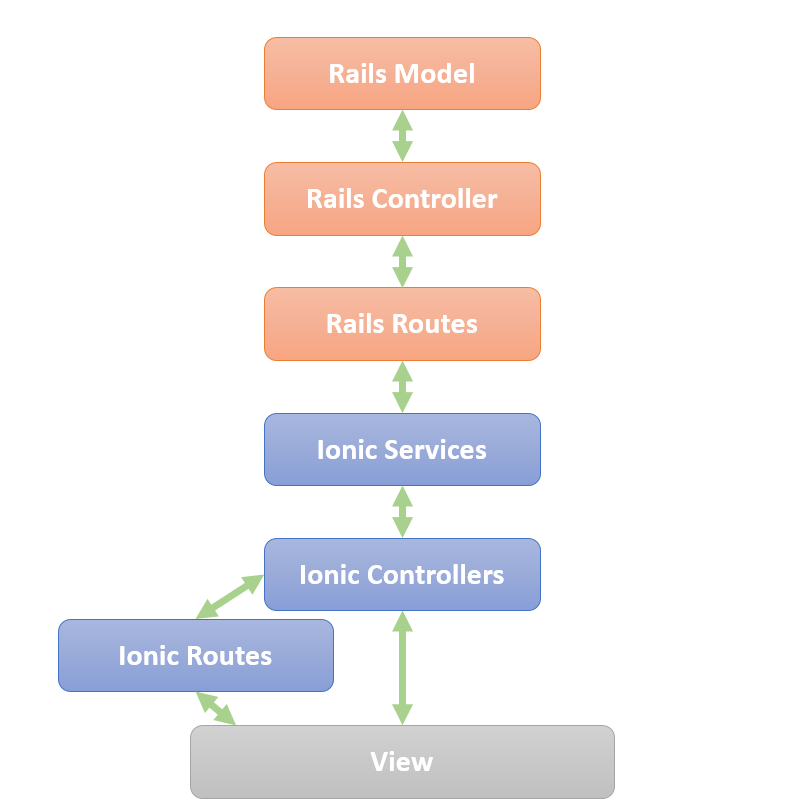
\includegraphics[width=10cm]{figuras/tecnologias}
\end{figure}

\par A camada Model é o lugar onde os dados são estruturados, consultados e validados. Ela se conecta diretamente com a camada de controle, pois a camada de controle que, através do input da camada de visão, irá definir quais dados serão consultados para que a camada de modelo faça conexão com a base de dados, e retorne sua resposta baseando-se nos dados analisados ou alterados.
\par A camada View é a responsável por todas as interações com o usuário e também fará contato com a camada de controle para definir quais informações serão mostradas para o usuário. As principais funções da camada de visão são mostrar a interface gráfica para os usuários e fazer a comunicação com a camada de controle.
\par Por usarmos o framework Ionic, são criadas as camadas Ionic Services, Ionic Controllers e Ionic Routes que implementam as funções de interface e portanto, a portabilidade da aplicação para sistemas Android, iOS, Windows Phone e Web.
\par A camada Controller é a camada que faz a ligação entre usuário e os dados, tendo vital importância dentro da arquitetura de nosso sistema. Os principais métodos que serão implementados estão na camada de controle. Para que essa camada execute os métodos ela recebe os comandos passados pelo usuário através da camada de visão e manipula os dados recebidos da camada de modelo. Para realizar todas as ações e navegação no sistema, esta camada utiliza das rotas da aplicação, na figura representada como a camada Rails Routes, para realizar suas funções.

\subsubsection{Tratamento de Dados}
\par Os dados a serem manipulados pelo software de controle serão recebidos do sistema de automação continuamente no formato de strings (conjuntos de caracteres, semelhante a texto). Estes dados serão armazenados no banco de dados do sistema e serão utilizados de acordo com as necessidades do usuário.
\par Caso o usuário utilize de algum recurso do software que precise do sistema de automação para ser realizado, como por exemplo, apagar a luz da garagem, o software de controle enviará comandos para o sistema de automação para que o mesmo realize a tarefa e mande de volta uma resposta.
\par Segue abaixo uma breve representação da transmissão de dados e da comunicação dos sistemas.

\begin{figure}[!h]
\centering
\caption{Representação da transmissão de dados e da comunicação dos sistemas}
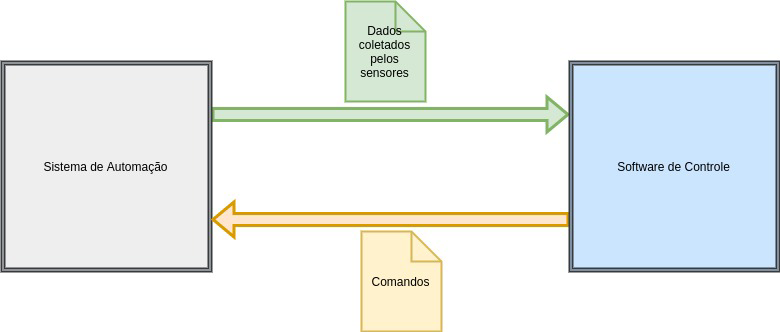
\includegraphics[width=10cm]{figuras/componentes}
\end{figure}

\subsection{Logo do Aplicativo}

\begin{figure}[!h]
\centering
\caption{Logo do Aplicativo}
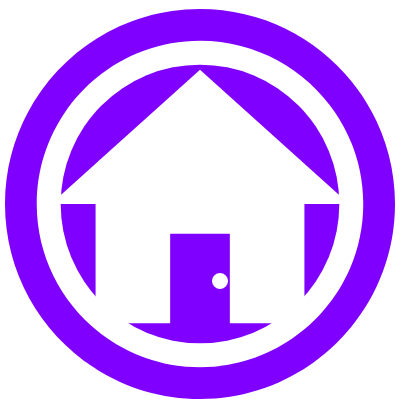
\includegraphics[width=5cm]{figuras/pi1}
\end{figure}

\subsection{Interface Com o Usuário}

\subsubsection{Tela Inicial}

\begin{figure}[!h]
\centering
\caption{Tela inicial do aplicativo}
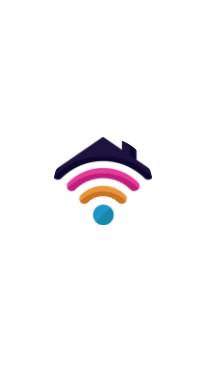
\includegraphics[width=5cm]{figuras/splash_screen}
\end{figure}

\par Mais conhecida como Splash Screen, nada mais é que uma tela que possui o ícone do Aplicativo e geralmente mostrada ao iniciar o aplicativo enquanto alguns dados referentes ao mesmo estão sendo carregados por trás.

\subsubsection{Tela de Login}

\begin{figure}[!h]
\centering
\caption{Tela de Login do Aplicativo}
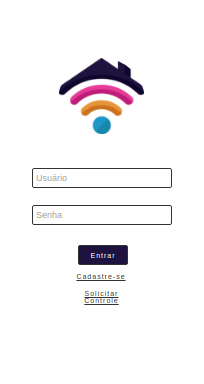
\includegraphics[width=5cm]{figuras/login}
\end{figure}

\par Tela para permitir que os usuários cadastrados realizem login no aplicativo.

\subsubsection{Painel Administrativo}

\begin{figure}[!h]
\centering
\caption{Painel Administrativo do Aplicativo}
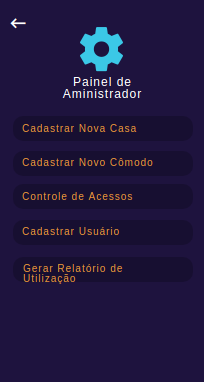
\includegraphics[width=5cm]{figuras/painel_adm}
\end{figure}

\par Painel responsável por permitir que o administrador gerencie toda a residência, seus cômodos e sensores.
\par Essa tela permite que o administrador realize todas as atividades que estão ligadas à esse perfil de usuário.

\subsubsection{Tela de Cadastro da Casa}

\begin{figure}[!h]
\centering
\caption{Tela de Cadastro da Casa}
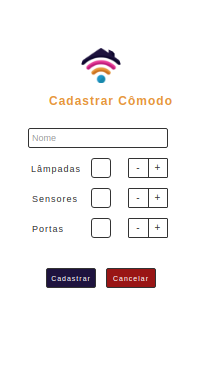
\includegraphics[width=5cm]{figuras/cadastro_casa}
\end{figure}

\par Tela responsável por permitir o cadastro de uma nova residência no sistema de controle inteligente.
\par Basta o usuário entrar com os dados da casa e já será possível realizar o controle da mesma.

\subsubsection{Tela de Cadastro do Usuário}

\begin{figure}[!h]
\centering
\caption{Tela de Cadastro do Usuário}
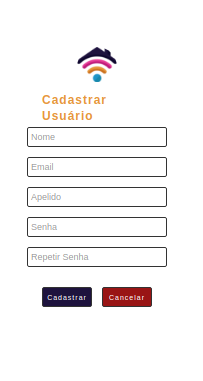
\includegraphics[width=5cm]{figuras/cadastro_de_usuario}
\end{figure}

\par Tela responsável por permitir que um novo usuário se cadastre no sistema.
\par Nela, basta que o mesmo entre com seus dados e se cadastre no software de controle de casa.

\subsubsection{Tela de Solicitar Controle da Casa}

\begin{figure}[!h]
\centering
\caption{Tela de Solicitar Controle da Casa}
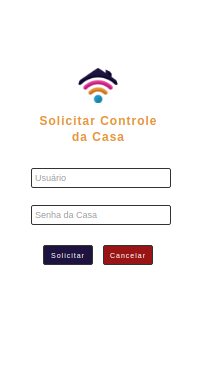
\includegraphics[width=5cm]{figuras/solicitar_controle}
\end{figure}

\par Tela que permite que um novo usuário solicite o controle e acesso à uma residência em específico.

\subsubsection{Tela de Controle de Acesso}

\begin{figure}[!h]
\centering
\caption{Tela de Controle de Acesso}
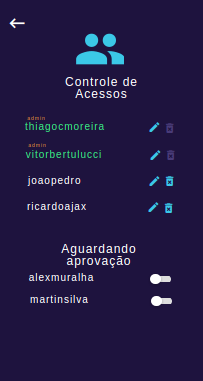
\includegraphics[width=5cm]{figuras/controle_acesso_casa}
\end{figure}

\par Permite gerenciar todo o controle de acesso à casa.
\par É uma tela específica para os administradores da casa, os quais podem editar quais os usuários responsáveis por poder gerenciar e controlar a casa por meio do aplicativo.

\subsubsection{Tela do Menu Inicial}

\begin{figure}[!h]
\centering
\caption{Tela do Menu Inicial}
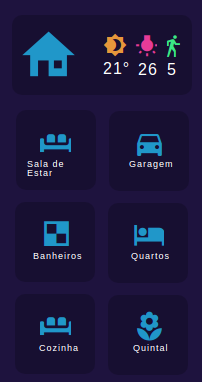
\includegraphics[width=5cm]{figuras/menu_inicial}
\end{figure}

\par Tela de menu inicial da casa, mostrando os cômodos cadastrados, bem como algumas informações gerais sobre os controladores da residência.

\subsubsection{Tela de Controle do Cômodo}

\begin{figure}[!h]
\centering
\caption{Tela de Controle do Cômodo}
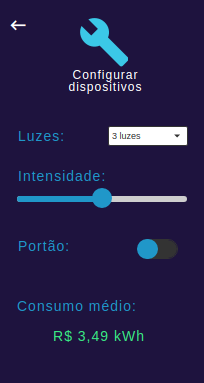
\includegraphics[width=5cm]{figuras/controle_comodo}
\end{figure}

\par Permite controlar os sensores e demais mecanismos controláveis de um cômodo em específico da residência.

\subsubsection{Tela dos Sensores do Cômodo}

\begin{figure}[!h]
\centering
\caption{Tela dos Sensores do Cômodo}
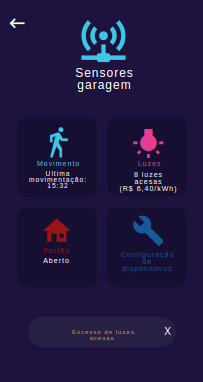
\includegraphics[width=5cm]{figuras/sensores_comodo}
\end{figure}

\par Tela que permite que o usuário com os devidos acessos à residência possa realizar o controle dos sensores de um cômodo em específico.

\subsubsection{Tela do Cômodo Específico}

\begin{figure}[!h]
\centering
\caption{Tela do Cômodo Específico}
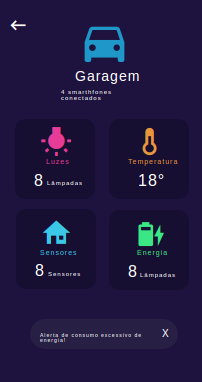
\includegraphics[width=5cm]{figuras/comodo_especifico}
\end{figure}

\par Permite visualizar as informações úteis referente à um cômodo em específico, desde que o mesmo já esteja cadastrado na casa.

\subsubsection{Tela da Visão Geral da Casa}

\begin{figure}[!h]
\centering
\caption{Tela da Visão Geral da Casa}
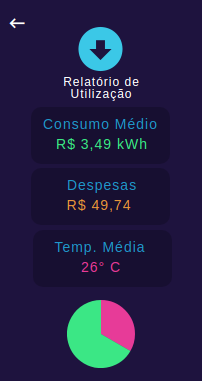
\includegraphics[width=5cm]{figuras/overview_casa}
\end{figure}

\par Tela responsável por mostrar de maneira clara uma visão genérica referente aos dados que estão sendo coletados pelos sensores instalados na casa, bem como os gastos totais até o momento e valores médios de consumo de enegia e afins.
